\chapter{Indledning}

I løbet af de seneste år er der sket en stor udvikling inden for digitalisering af samfundet og dets arbejdsprocessor\cite{Erhverv}. Denne digitale udvikling ønsker de også hos Rambøll. De vil gerne væk fra at skulle have papirstegninger med ud på byggepladsen for at tage notater til et byggeprojekt. \\
I dag er der flere ansatte ved Rambøll som har papir og blyant med ud på byggepladsen for at registre deres observationer. Derfor ønsker Rambøll at få udviklet en applikation, som kan gøre denne arbejdsproces nemmere.
Der er blevet udviklet en prototype i form af en applikation med navn Rambøll Tilsyn til dette formål.
Rambøll Tilsyn består af en applikation med en tilhørende database, som det kan ses på oversigten på Figur \ref{fig:OversigtSystembeskrivelse}


\begin{figure}[H]
	\centering
	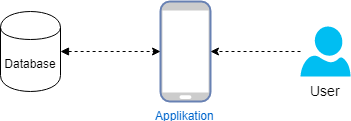
\includegraphics[width=0.4\linewidth]{Indledning/Oversigtoversystem}
	\caption{Oversigt over systemet.}
	\label{fig:OversigtSystembeskrivelse}
\end{figure}

Med dette system vil de ansatte hos Rambøll kunne lave deres registreringer direkte i applikationen og derved bliver de fri for at bruge papir og blyant. \\

\section*{Ansvarsområder}
Tabel \ref{Produktansvar} viser en overordnet fordeling af ansvarsområderne i udvikling af produktet Rambøll Tilsyn. Kravspecifikationen er blevet udarbejdet af gruppen i samarbejde med Rambøll. \\

\begin{table}[H]
	\centering
	\begin{tabular}{lllll} \hline
		\textbf{Ansvar} &  & \textbf{Ao}&  \textbf{Morten}&  \\ \hline
		Back-end&  &  X&  &  \\ \hline
		Applikation&  &  X&  X&  \\ \hline
		Dokumentation& & & X& \\ \hline
	\end{tabular}
	\caption{Ansvarsområder for udvikling.}
	\label{Produktansvar}
\end{table}